\documentclass[12pt,a4paper]{article}

\usepackage[T1]{fontenc}
\usepackage[utf8]{inputenc}
\usepackage[brazil]{babel}
\usepackage{lmodern}
\usepackage[a4paper,margin=2.5cm]{geometry}
\usepackage{setspace}
\usepackage{graphicx}
\usepackage{float}
\usepackage[hidelinks]{hyperref}

\onehalfspacing

\graphicspath{{results/}{report/results/}}

\title{\textbf{Análise de desempenho das versões sequencial, OpenMP e MPI do problema de isomorfismo em grafos}}
\author{Pedro Gabriel do Valle Nogueira}
\date{\today}

\begin{document}

\maketitle

\section{Objetivo}

Este relatório compara o desempenho de três implementações do mesmo algoritmo:

\begin{itemize}
    \item \textbf{Sequencial}: versão base, usada como referência.
    \item \textbf{OpenMP}: versão paralela com \textit{threads}.
    \item \textbf{MPI}: versão paralela com processos.
\end{itemize}

O foco da análise é o tempo médio de execução e o \textit{speedup} das versões paralelas em relação à versão sequencial.

\section{Configuração dos Testes}

Os testes foram executados com \texttt{N} repetições para cada entrada. Para comparar OpenMP e MPI de forma equivalente, o número de \textit{threads} do OpenMP foi configurado para ser igual ao número de processos do MPI.

\begin{itemize}
    \item Número de repetições: \texttt{N = preencher}
    \item Número de \textit{threads}/processos: \texttt{P = preencher}
    \item Máquina utilizada: \texttt{preencher}
    \item Compilação: \texttt{-O3}; OpenMP com \texttt{-fopenmp}; MPI com \texttt{mpicc}
\end{itemize}

Os resultados brutos foram gerados pelo script \texttt{benchmark.py} e salvos em \texttt{results.csv}. As figuras foram geradas a partir desse arquivo.

\section{Resultados}

A Figura~\ref{fig:runtime} mostra o tempo médio de execução para cada entrada. As barras de erro representam o desvio padrão entre as repetições.

\begin{figure}[H]
    \centering
    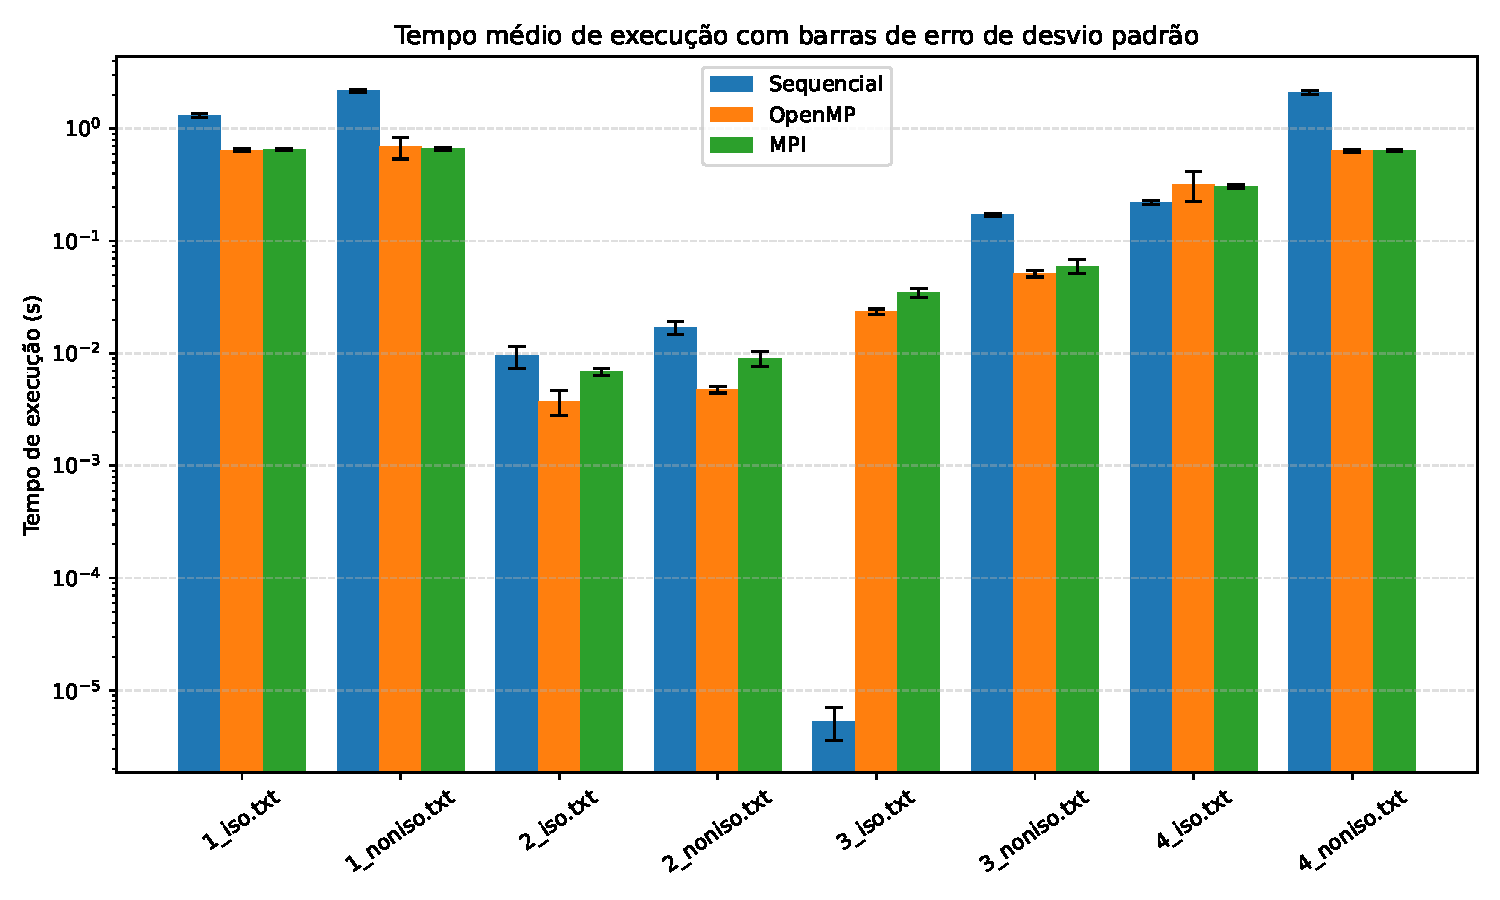
\includegraphics[width=0.95\textwidth]{runtime_errorbars.pdf}
    \caption{Tempo médio de execução das versões sequencial, OpenMP e MPI.}
    \label{fig:runtime}
\end{figure}

A Figura~\ref{fig:speedup} mostra o \textit{speedup} das versões paralelas em relação à versão sequencial. As barras de erro representam o desvio padrão dos valores de \textit{speedup} calculados em cada repetição.

\begin{figure}[H]
    \centering
    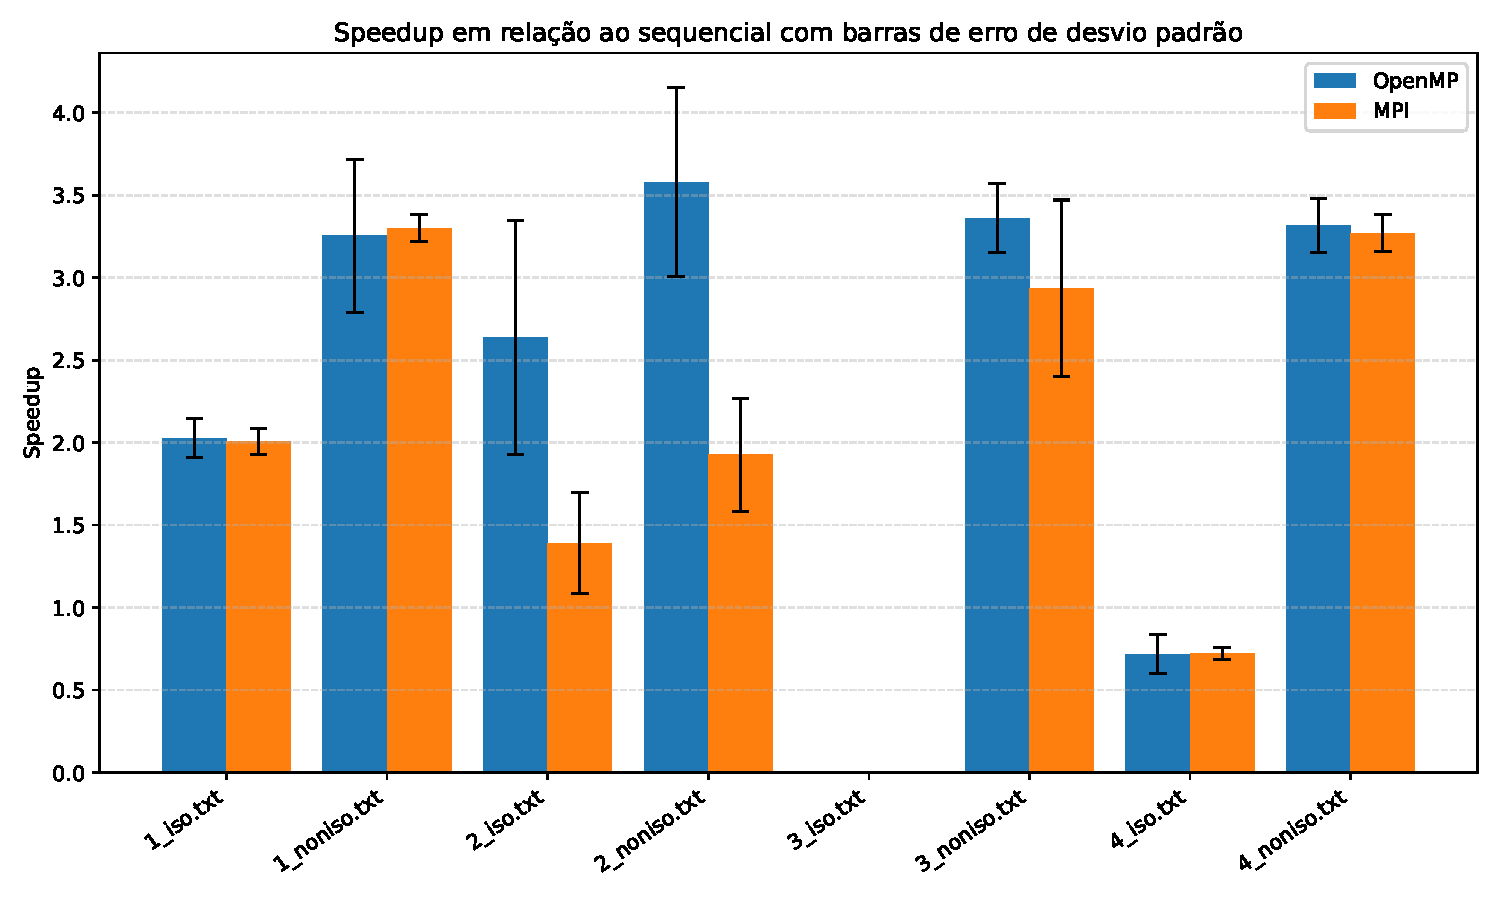
\includegraphics[width=0.95\textwidth]{speedup_errorbars.pdf}
    \caption{\textit{Speedup} das versões OpenMP e MPI em relação à versão sequencial.}
    \label{fig:speedup}
\end{figure}

\section{Análise}

Preencha esta seção com a interpretação direta dos resultados. Sugestão de pontos a comentar:

\begin{itemize}
    \item Em quais entradas OpenMP teve melhor desempenho.
    \item Em quais entradas MPI teve melhor desempenho.
    \item Se houve casos em que o paralelismo piorou o desempenho.
    \item Relação entre tamanho da entrada e ganho de desempenho.
    \item Possíveis causas de sobrecusto: criação de \textit{threads}, comunicação MPI, sincronização e parada antecipada.
\end{itemize}

\section{Conclusão}

Resumo curto dos resultados principais:

\begin{itemize}
    \item Melhor abordagem observada: \texttt{preencher}.
    \item Entradas em que o paralelismo foi vantajoso: \texttt{preencher}.
    \item Entradas em que o paralelismo não compensou: \texttt{preencher}.
\end{itemize}

\end{document}
